\documentclass[a4paper,10pt]{report}
\usepackage{hyperref}
\usepackage{graphicx}
\usepackage{wrapfig}
\graphicspath{ {Diagrams/} }
\hypersetup{
    colorlinks=true,
    linkcolor=blue,
    filecolor=magenta,
    urlcolor=cyan,
}

\newcommand{\code}{\texttt}

% Title Page
\title{
Benchmarking application for Android
}
\author{Peter-Tibor Zavaczki, 30433}
\date{march 14, 2018}


\begin{document}
\maketitle

\chapter{Introduction}
\section{About}
 \subsection{Benchmarking}
 The procedure of benchmarking describes running some set of programs on a system to evaluate the performance of said system. When the term refers to assessing hardware, the most commonly tested element is the CPU, the GPU, RAM and storage drive tests being the less common, yet still seen parts of benchmarks. Testing the CPU relies on, among others, running some very resource consuming algorithms in a closed environment and measuring their execution time, then based on an arbitarily set standard, grading the device.
 \subsection{Android}
 Android is a monolithic operating system based on a modified version of the Linux kernel, its core being written mainly in C and C++, while its UI is written in Java.

 There are some less known programming languages, such as Kotlin and Go, which are used to develop Android applications, bust most of them are developed in Java, which will be the case for this project aswell. The most essential part of developing an Android application is the Android SDK, which is also written in Java. The current official IDE to develop Android applications in is Android Studio, developed by Google and powered by IntelliJ, although since the code is Java, other Java based IDEs can be used aswell, such as Eclipse, IntelliJ or NetBeans. Compiled code is packaged in .apk type executables, which are stored in \code{/data/app} but it is only accessible to the root user for security reasons.

\newpage
\section{Specifications}
 \begin{itemize}
 \item The purpose of this project is to develop an application for Android, which shows concrete data about the device's capability to perform a certain task.
 \item The user's interaction with the application should be fairly restrained, he being able to start the benchmarking process and observing the final results after its completion.
 \item The application is designed to run on devices running Android OS, and being run in strictly in a local environment.
 \item The language used for coding is Java
 \item The application should run its test in as much of a closed environment as possible. % This means that, in the ideal case, the application should have exclusive and full access to the tested resource, such as being the only process running on a core of the CPU until the running algorithm finishes. Of course the previously stated example is very extreme, since the OS will always have higher priority than any user application and as such our users application's process will most likely be constantly interrupted by the OS for it to perform its own actions.
 \end{itemize}

\section{Topic inquiry}
 For the development of this project I have to look into the targeted topic and familiarize myself with, developing software for Android and coming up with stable and reliable benchmarks.

 The articles read were:
 \begin{enumerate}
 \item \href{https://www.androidauthority.com/write-an-android-cpu-benchmark-part-1-679929/}{''Create a CPU benchmark tool''}, by Adam Sinicki
 \item \href{https://www.androidauthority.com/write-an-android-cpu-benchmark-tool-part-2-681455/}{''How to write an Android benchmark''}, by Adam Sinicki
 \end{enumerate}

 \subsubsection{''Create a CPU benchmark tool'', by Adam Sinicki}
 This article introduces the basics of benchmarking by explaining the concept that we need to run heavy algorithms to stress the CPU, and that the execution time may differ because of the ongoing processes in the background. Then it goes on explaining the basics behind SHA-1 (Secure Hash Algorithm 1), formerly used to hash sensitive data. I say formerly, since newer computers as powerful enough so that brute force attack are an option to cracking the hash resulted from SHA-1; nowadays SHA-2, SHA-3 or other hashing algorithms are used for better security.

 The next topic is building the actual Android app. The UI's design is shown by the .xml file and the emulated result shown in the virtual Android device in Android Studio.

 After the author finished with creating the basic UI design, he goes on to develop the mechanics of the application, creating the functions to be called that measure the time it takes for the CPU to perform a certain action.
 
 Being finished with the basic hash function calling function, the author adds an event to a button, which when pressed executes the previously written hash function.
 
 Seeing as the code executes very fast, a simple for loop is added to repeat the hashing function 20000 times, thus drastically slowing down the complete execution process. 
 
 As a final touch the author decides to divide the result given in the nanoseconds taken to execute the hashing by 100000000 to get a grade in a reasonable scale.

 \subsubsection{''How to write an Android benchmark'', by Adam Sinicki}
 This article focuses on introducing more complex concepts to building a benchmark, such as the MD5 encryption protocol, multi threading the application, runnables and handlers.
 
 Firstly, a function for calculating the MD5 hash is created, the time for calling it 20000 times is measured, added to the time required to calculate 20000 SHA-1 hashes and an average is made for getting the grade for the device.
 
 After using the MD5 protocol to hash a string 20000 times, the author writes a simple for cycle to count to a $ 10^n $ . This part of his code represents the time it takes for the device to brute force crack an n-digit password. 
 
 The following step in the process of building the benchmark is multi threading the application. More specifically, the author creates a Runnable for the previously written 'brute force cracker' and runs it in a new thread. He relates that, unfortunately threads have no way of communicating between each other in of themselves and as such the time cannot be measured, nor can we know if the function finished or not. For this he uses a Handler, which sends a message containing the time it took to run the function in the Runnable.
 
 As a final note, the author adds that he moved every function to a separate thread and calculated the execution time for each of them separately, thus making it so the application and device didn't freeze while it ran its tests and getting a final grade for his device.

\chapter{Design}

\section{Construction}
 This project is created for Android OS running devices, thus Android Studio is used as the principal IDE. On the other side, Java is used for programming the back-end of the application and xml/css for the UI/front-end.
 
 \begin{figure}[h]
  \centering
  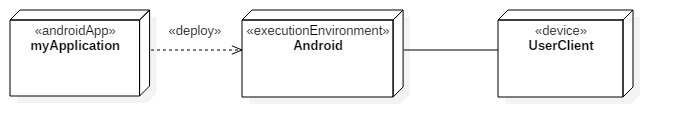
\includegraphics[width=0.5\textwidth]{DeploymentDiagram1.png}
  \caption{The deployment diagram of the project}
  \label{fig:deplDiag1}
 \end{figure}
 
 \section{Modules}
 
 \begin{wrapfigure}[13]{r}{0.25\textwidth}
  \centering
  \caption{}
  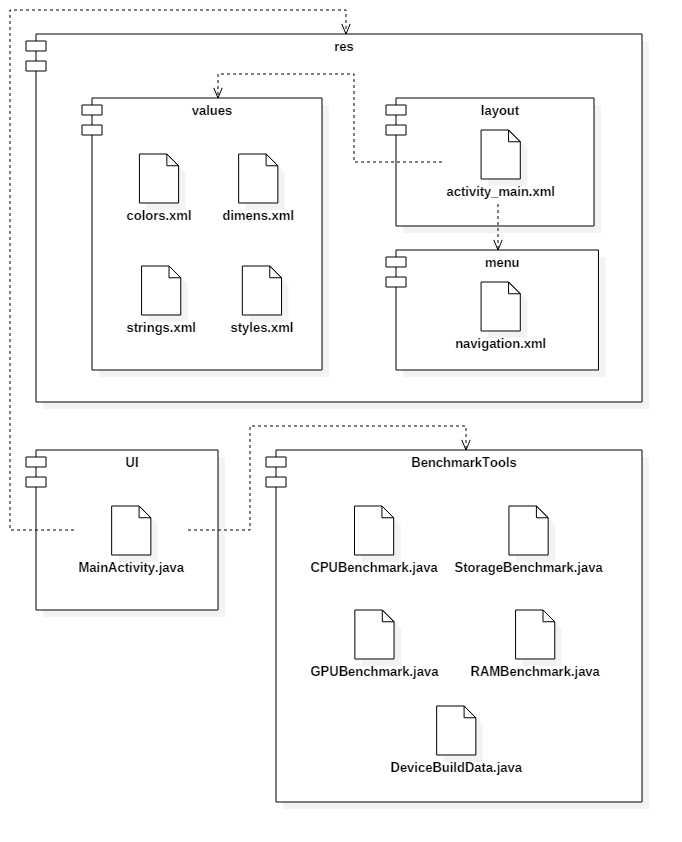
\includegraphics[width=0.5\textwidth]{ComponentDiagram1.png}
  \label{fig:compDiag1}
 \end{wrapfigure}
 
 The application will, of course be modularized based on two main categories, the front-end and the back-end, and then, based on the back-end point of view on several other modules based on the type of hardware resouce that is tested, such as CPU, GPU, storage etc. This can be seen on figure \ref{fig:compDiag1}, representing the component diagram of the project.
 
 \section{Testing}
 Since the application is modularized, automatic test can be implemented, such as JUnit tests, thank to the usage of Java. These tests can hold the whole project together and signal if there is an error in a module, in case we change something in a related module.
 
 \pagebreak
 \section{Benchmarking}
 The benchmark tests need to be specific for each hardware element we wish to test. For the CPU, heavy arythmetic operations will be performed several times, and an average execution time will be measured. For the GPU, a 3D graphically complex scene will be played and rendered, while the FPS (frames per second) is measured and averaged. For the storage unit, a large dummy file can be copied from one place to the other, thus measuring its mean speed.
 
 For the final calculations, and summation of all the data, we could take the sum of the milliseconds used to calculate everything, while creating an equation for calculating and approximate value for this point system for the GPU test aswell, with the average FPS count.
 
 \section{Use-cases}
  The user client can interact with the app in the following ways: he wishes to benchmark the device to see how it performs, or he wishes to see information about the device's hardware build. This use-case can be seen in figure \ref{fig:useCaseDiag1}.
  
 \begin{figure}[h]
  \centering
  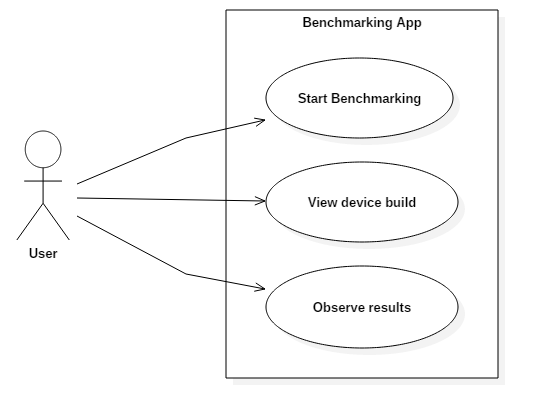
\includegraphics[width=0.5\textwidth]{UseCaseDiagram1.png}
  \caption{The use-case diagram for both possible actions of the actor}
  \label{fig:useCaseDiag1}
 \end{figure}
 
 \subsection{Use-case: Benchmarking the device}
 This use-case is active if the client user chooses to benchmark his device. He can choose this option by tapping the corresponding button. Following the button's tap, the application starts several processes, regarding the different component's benchmarking tasks, such as hashing a String with SHA-1 for the CPU. As a process completes, a message is displayed in the logging area notifying the user and displaying the score. This sequence of actions can be observed on figure \ref{fig:benchSeqDiag1}.
 
 \begin{figure}[h]
  \centering
  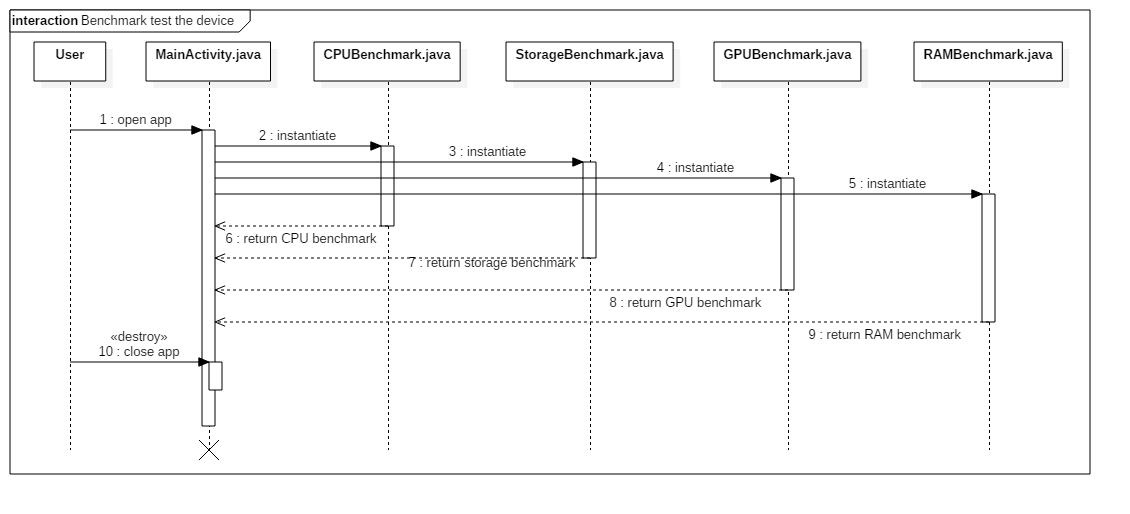
\includegraphics[width=0.9\textwidth]{SequenceDiagram_Benchmark.png}
  \caption{The sequence diagram representing the benchmarking process}
  \label{fig:benchSeqDiag1}
 \end{figure}
 
 \pagebreak
 \subsection{Use-case: Querying the device's hardware build}
 This use-case is active if the client user chooses to view his device's hardware build. He can do this by tapping the corresponding button. Following the button's tap, the application starts a process during which it queries, then displays the reuested information. This sequence of actions can be observed on figure \ref{fig:querySeqDiag1}.
 
 \begin{figure}[h]
  \centering
  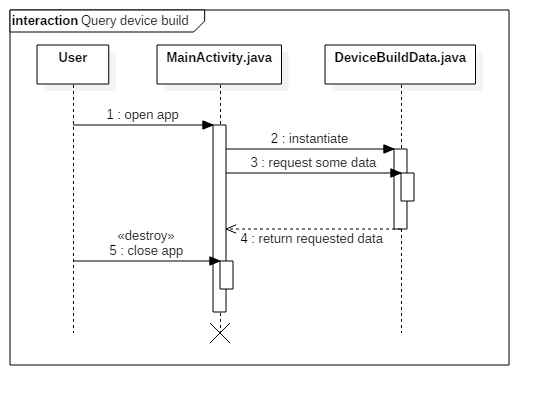
\includegraphics[width=0.5\textwidth]{SequenceDiagram_DeviceBuild.png}
  \caption{The sequence diagram representing the querying of the device's hardware}
  \label{fig:querySeqDiag1}
 \end{figure}
 
 \pagebreak
 \section{Packages}
 The application consists of only two packages: the BechmarkTools package, containing the different classes to run the benchmarking process' stages, and the com.example.peter.myapplication package, which is basically the package containing the UI layer of the application. This package diagram can be seen on figure \ref{fig:packageDiag1}.
 
 \begin{figure}[h]
  \centering
  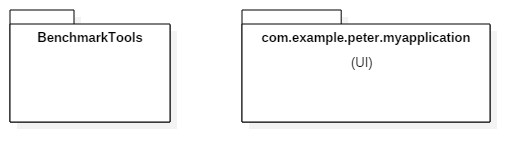
\includegraphics[width=0.5\textwidth]{PackageDiagram1.png}
  \caption{The package diagram of the project}
  \label{fig:packageDiag1}
  
 \end{figure}

\chapter{Implementation}
 \section{The environment}
 This proposed project deals with making a basic CPU benchmarking tool and querying some basic information about the mobile device's build.\\
 The tools and technologies used for achieving this task are programming in Android, which relies on Java, with the Android Studio dedicated IDE, developed with Google, powered by JetBrains' IntelliJ.\\
 
 \section{Architecture}
 The built project, due to it being written mainly in Android, is based on an MVC architectural model.\\
 The models are defined in the benchmarkTools package, the view being the UI, defined using the layout xml files and the controllers are the .java files which contain the word Activity in their name.\\
 The model is composed of two files: CPUBenchmark.java and DeviceInfo.java.\\
 CPUBenchmark.java contains the functions which test the CPU's power, by measuring the time it takes to measure hashing a string with SHA-1 algorithm, measuring the FLOPS (Floating Point Operations Per Second) and the MIPS (Millions of Instruction Per Second).\\
 DeviceInfo.java contains the functions which query the basic device build and another function which tells the number of cores on the CPU.\\
 The controller is just one class MainActivity.java, which contains the main function used for the Android lifecycle and the listener for the botton navigation bar, within which the adequate functions are called to display data on screen.\\
 The view, defined in the layout folder within resources, contains an xml definition of a hierarchically built view.\\
 
 \section{Tests}
 \subsection{SHA-1 processing}
 SHA-1 stands for Secure Hash Algorithm, it is a cryptographic hash function which takes an input and produces a 160-bit (20-byte) hash value known as a message digest - typically rendered as a hexadecimal number, 40 digits long.\\
 In this project we calculate the SHA-1 value of a string from the res/values/strings.xml, called string\_to\_hash.\\
 This is done by including the MessageDigest class from java's security package, creating an instance of it by specifying the task it will be used for is hashing things with SHA-1.\\
 By calling the digest() function we get the result of digesting the input string in a byte array.\\
 The previously received byte array is then processed by transforming each byte into a string value and appending it to the output string.\\
 This process trasforms the input string "Swiggity swooty im coming for that passing mark!" into the output string "ed446da10ca83eee3dd9122cc474e01cc4b9a25e".\\
 Then, the time taken to process this operation is measured and displayed in the UI.
 
 \subsection{FLOPS count}
 FLOPS stands for Floating Point Operations Per Second and it is a measure of computer performance, useful in fields of scientific computations that require floating-point calculations..\\
 For the FLOPS test I run several operations on double type variable and count the time for each of them sepparately, at the end returning the sum of the time taken to do all the operations.\\
 The time is counted in nanoseconds for a higher precision.\\
 The operations performed are multiplication, additon, negation, division, subtraction, conversion to long (non floating point type represented on 64 bits) and conversion of the long variable back to double.\\
 These 7 total operations' processing times, being in nanoseconds are summed up and returned out of the function, being then processed in the calling function which calculated the FLOPS from the previously returned data.\\
 The FLOPS of the CPU is calculated as follows: the previous result is divided 1000000000, since it was in nanoseconds and we want to show in how many seconds has the 7 operations been done.\\
 Then we divide 7 by that value so we get X floating point operations are done in 1 second, this being the definition of FLOPS.\\
 
 \subsection{MIPS count}
 IPS stands for Onstructions Per Second and is a measure of a computer's processor performance.\\
 Since modern processors are quite powerful, counting IPS returns a high number, so it is a common approach to count thousands (TIPS/KIPS), millions (MIPS) of billions of IPS (GIPS).\\
 In our tests, we use MIPS.\\
 The MIPS test is done similarly to how the FLOPS test is done. \\
 Seven operations are performed on an integer type variable (add, sub, mul, div, neg, convert to float, convert float to int) with counting the time it takes for each of these operations to be completed and then at the end the sum of these times are returned.\\
 The time is counted in nanoseconds for a higher precision.\\
 This returned value is processed in a different function, where from the nanoseconds it took to perform these 7 ops we get a MIPS value.\\
 This is done by dividing the returned time with 1000000000 to get the value in seconds, then we divide 7 with the resulting value, getting the IPS of the processor, the divide it all with 1000000 to get the final MIPS value, which is then returned to be displayed on the UI.\\
 
 \section{Querying the device's build}
 The querying of the device's build is maily done by using the Build class of the os package from adroid's packages.\\
 There are some values in this class which can be accessed statically, thus calling \textit{Build.MANUFACTURER} will give us the manufacturer, which is noted in the device's datasheet, accessed by the Build class.\\
 The values outputted are the manufacturer, the model, the brand, the board, the display, the device, the fingerprint and the hardware informations.\\
 The final value outputted is the number of cores on the CPU.\\
 This value is calculated by having a function, called getNumCores, which has an inner class CpuFilter defined, which looks for files in the /sys/devices/system/cpu/ of the format "cpu[0-9]+".\\
 The number of such files found will be the number of cores on the CPU.\\
 
\chapter{Summing up}
 \section{Results}
 The main result of this project was the 
 

\end{document}
